% Fuse: a per-stream reliable transport over UDP -- CS3530 presentation (15 minutes, 20 slides).
% Build:  latexmk -lualatex presentation.tex   (LuaLaTeX; JetBrains Mono is bundled in fonts/)

\documentclass[aspectratio=169,11pt]{beamer}
\setbeamertemplate{navigation symbols}{}
\setbeamertemplate{footline}[frame number]
\setbeamertemplate{itemize items}[circle]
\setbeamertemplate{blocks}[rounded][shadow=false]

% No hyphenation: the slides must contain no '-' characters at all.
\hyphenpenalty=10000 \exhyphenpenalty=10000 \uchyph=0
\usepackage{fontspec}
\setmonofont{JetBrainsMono}[
  Path=fonts/, Extension=.ttf, UprightFont=*-Regular, BoldFont=*-Bold,
  ItalicFont=*-Italic, BoldItalicFont=*-BoldItalic, Scale=0.88]
\usepackage{booktabs,multirow}
\usepackage{tikz}
\usetikzlibrary{arrows.meta,positioning,calc,fit,shapes.geometric,decorations.pathreplacing}

\definecolor{fblue}{RGB}{31,94,165}
\definecolor{fred}{RGB}{192,57,43}
\definecolor{fgreen}{RGB}{35,134,54}
\definecolor{fgray}{RGB}{110,110,110}
\setbeamercolor{frametitle}{fg=fblue}
\setbeamercolor{title}{fg=fblue}
\setbeamercolor{structure}{fg=fblue}
\setbeamercolor{block title}{fg=white,bg=fblue}
\setbeamercolor{block body}{bg=fblue!6}

\tikzset{
  box/.style={draw=fgray, rounded corners=2pt, align=center, font=\footnotesize, inner sep=3pt, fill=white},
  bbox/.style={box, draw=fblue, fill=fblue!8},
  rbox/.style={box, draw=fred, fill=fred!8},
  gbox/.style={box, draw=fgreen, fill=fgreen!8},
  arr/.style={-{Stealth[length=2mm]}, thick},
  msg/.style={-{Stealth[length=1.8mm]}, semithick},
  lost/.style={msg, dashed, fred},
  lab/.style={font=\scriptsize, align=center},
}
\newcommand{\fitwidth}[1]{\resizebox{\ifdim\width>\linewidth\linewidth\else\width\fi}{!}{#1}}
\newcommand{\rf}[1]{{\scriptsize\,[#1]}}
% Two boxes used on the protocol slides.
\newcommand{\happening}[1]{\begin{block}{What is happening}\scriptsize #1\end{block}}
\newcommand{\better}[1]{\begin{block}{Where we are better}\scriptsize #1\end{block}}

% ---- Measured results -------------------------------------------------------------------------
% (a) bench/RESULTS.md, 16 core host, protocol v5-v7, 1 GiB, unencrypted.
% (b) this project's re run on a 12 core laptop, protocol v8, 512 MiB, loopback, median of 3.
% Numbers measured for the presentation (CS3530) on a 12 core Linux laptop, protocol v8, loopback.
% Throughput: 512 MiB in memory, median of 3 runs. Latency: 64 byte probes at 2000/s for 5 s,
% 4 bulk streams. Reliability: 32 MiB through bench/fuse_netem. QUIC numbers on the slides are quoted
% from bench/RESULTS.md (16 core host, protocol v5 to v7).
\newcommand{\FUSEONE}{1318}     % Fuse, 1 lane, MB/s
\newcommand{\FUSEFOUR}{1070}    % Fuse, 4 lanes
\newcommand{\TCPONE}{6023}      % TCP, 1 connection
\newcommand{\TCPFOUR}{5189}     % TCP, 4 connections
\newcommand{\UDPRAW}{552}       % raw UDP send rate (no reliability)
\newcommand{\UDPDELTWO}{48.2}   % raw UDP, % of datagrams delivered through 2% emulated loss, sent at line rate
\newcommand{\UDPDELFIVE}{46.3}  % same, 5% loss
\newcommand{\FUSELATIDLEA}{30.1}  \newcommand{\FUSELATIDLEB}{136.6}  % Fuse idle p50 / p99 (us)
\newcommand{\FUSELATLOADA}{19.2}  \newcommand{\FUSELATLOADB}{188.0}  % Fuse under 4 lane bulk (5.5 GB/s)
\newcommand{\TCPLATIDLEA}{40.8}   \newcommand{\TCPLATIDLEB}{130.6}   % TCP idle
\newcommand{\TCPLATSAMEA}{15.0}   \newcommand{\TCPLATSAMEB}{15015.9} % TCP, probes on a bulk connection
\newcommand{\TCPLATSEPA}{25.2}    \newcommand{\TCPLATSEPB}{835.6}    % TCP, probes on their own connection
\newcommand{\QUICJIT}{0.6}      % QUIC MB/s under 10+/5 ms jitter (bench/RESULTS.md)
\newcommand{\FUSEJIT}{50}       % Fuse MB/s under the same jitter (bench/RESULTS.md)


\title{Fuse}
\subtitle{A reliable transport over UDP, stream by stream}
\author{Boreddy Sri Sai Abhinav Reddy \quad\textbar\quad Chiruvella Gagan Chandra Sai Ram\\[2pt]
        Kamal Koushik Duppalapadi \quad\textbar\quad Tavva Dinesh Reddy}
\institute{CS3530: Computer Networks}
\date{}

\begin{document}

% 1 ------------------------------------------------------------------------------------------------
\begin{frame}[plain]
  \titlepage
\end{frame}

% 2 ------------------------------------------------------------------------------------------------
\begin{frame}{Problem statement}
  \begin{center}
    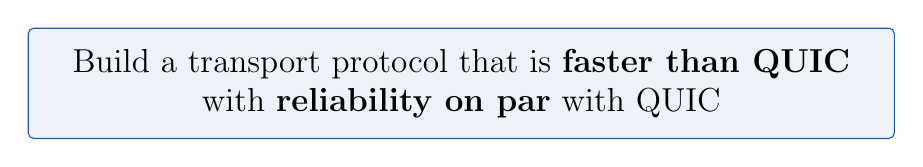
\begin{tikzpicture}
      \node[bbox, minimum width=11cm, minimum height=1.4cm, font=\large] (p)
        {Build a transport protocol that is \textbf{faster than QUIC}\\ with \textbf{reliability on par} with QUIC};
    \end{tikzpicture}
  \end{center}
  \vspace{4mm}
  \begin{columns}[T]
    \column{0.47\textwidth}
    \textbf{Faster}
    \begin{itemize}\small
      \item higher throughput for large objects
      \item low, flat latency for small messages \emph{while} bulk data flows
      \item graceful under loss, jitter and reordering
    \end{itemize}
    \column{0.47\textwidth}
    \textbf{Reliable}
    \begin{itemize}\small
      \item every byte delivered, in place, verified
      \item recovers from loss, duplication, reordering
      \item optional authenticated encryption (AES GCM)
    \end{itemize}
  \end{columns}
\end{frame}

% 3 ------------------------------------------------------------------------------------------------
\begin{frame}{Why this problem?}
  \centering
  \fitwidth{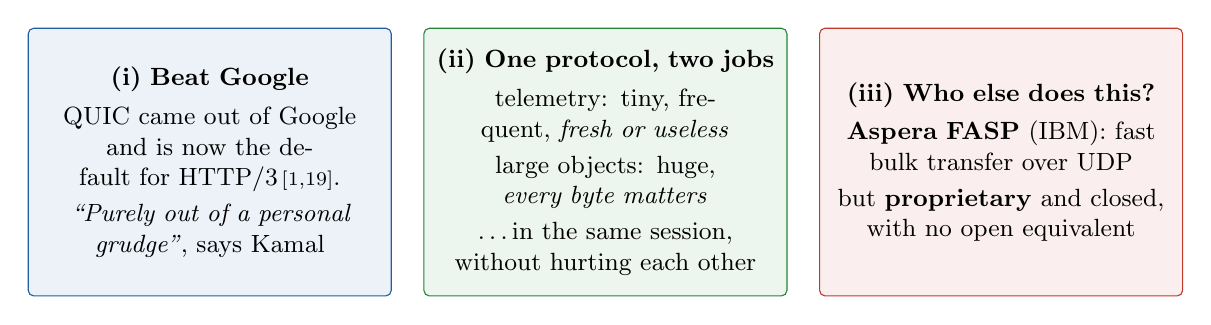
\begin{tikzpicture}[node distance=4mm]
    \node[bbox, text width=4.4cm, minimum height=3.4cm, font=\small] (a) {\textbf{(i) Beat Google}\\[3pt]
      QUIC came out of Google and is now the default for HTTP/3\rf{1,19}.\\[2pt]
      \emph{``Purely out of a personal grudge''}, says Kamal};
    \node[gbox, text width=4.4cm, minimum height=3.4cm, font=\small, right=of a] (b) {\textbf{(ii) One protocol, two jobs}\\[3pt]
      telemetry: tiny, frequent, \emph{fresh or useless}\\[2pt]
      large objects: huge, \emph{every byte matters}\\[2pt]
      \dots in the same session, without hurting each other};
    \node[rbox, text width=4.4cm, minimum height=3.4cm, font=\small, right=of b] (c) {\textbf{(iii) Who else does this?}\\[3pt]
      \textbf{Aspera FASP} (IBM): fast bulk transfer over UDP\\[2pt]
      but \textbf{proprietary} and closed, with no open equivalent};
  \end{tikzpicture}}
  \vspace{5mm}

  \small(iv) and QUIC itself has pitfalls for this mix $\Rightarrow$ next slide
\end{frame}

% 4 ------------------------------------------------------------------------------------------------
\begin{frame}{Pitfalls of QUIC (which we address)}
  \centering
  \fitwidth{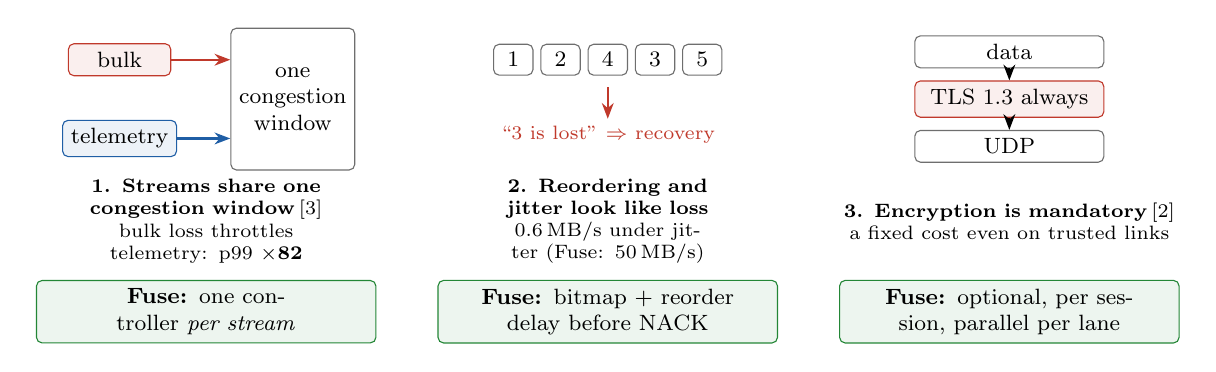
\begin{tikzpicture}
    % 1: shared congestion window
    \node[rbox, minimum width=1.3cm] (b1) at (0,1.2) {bulk};
    \node[bbox, minimum width=1.3cm] (t1) at (0,0.2) {telemetry};
    \node[box, minimum height=1.8cm, minimum width=1.4cm] (w1) at (2.2,0.7) {one\\congestion\\window};
    \draw[arr, fred] (b1) -- (w1.west|-b1); \draw[arr, fblue] (t1) -- (w1.west|-t1);
    \node[lab, text width=4.3cm] at (1.1,-0.85) {\textbf{1. Streams share one congestion window}\rf{3}\\
      bulk loss throttles telemetry: p99 \textbf{$\times$82}};
    \node[gbox, text width=4.1cm] at (1.1,-2.0) {\textbf{Fuse:} one controller \emph{per stream}};
    % 2: reordering read as loss
    \foreach \x/\n in {0/1,0.6/2,1.2/4,1.8/3,2.4/5} \node[box, minimum width=5mm] at (5+\x,1.2) {\n};
    \draw[arr, fred] (6.2,0.85) -- (6.2,0.45);
    \node[lab, text=fred] at (6.2,0.25) {``3 is lost'' $\Rightarrow$ recovery};
    \node[lab, text width=4.3cm] at (6.2,-0.85) {\textbf{2. Reordering and jitter look like loss}\\
      \QUICJIT\,MB/s under jitter (Fuse: \FUSEJIT\,MB/s)};
    \node[gbox, text width=4.1cm] at (6.2,-2.0) {\textbf{Fuse:} bitmap + reorder delay before NACK};
    % 3: mandatory TLS
    \node[box, minimum width=2.4cm] (app) at (11.3,1.3) {data};
    \node[rbox, minimum width=2.4cm] (tls) at (11.3,0.7) {TLS 1.3 always};
    \node[box, minimum width=2.4cm] (udp) at (11.3,0.1) {UDP};
    \draw[arr] (app) -- (tls); \draw[arr] (tls) -- (udp);
    \node[lab, text width=4.3cm] at (11.3,-0.85) {\textbf{3. Encryption is mandatory}\rf{2}\\
      a fixed cost even on trusted links};
    \node[gbox, text width=4.1cm] at (11.3,-2.0) {\textbf{Fuse:} optional, per session, parallel per lane};
  \end{tikzpicture}}
\end{frame}

% 5 ------------------------------------------------------------------------------------------------
\begin{frame}{How? Have you ever used IDM?}
  \begin{columns}[c]
    \column{0.55\textwidth}
    \centering
    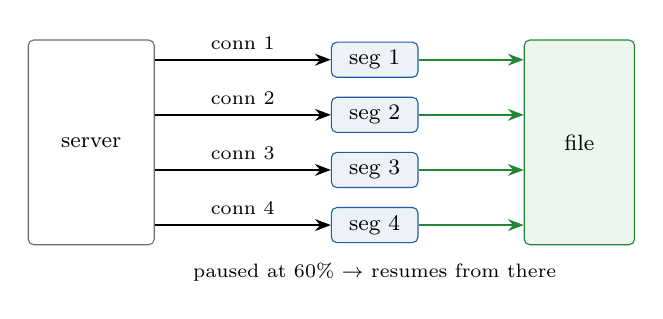
\begin{tikzpicture}
      \node[box, minimum width=1.6cm, minimum height=2.6cm] (srv) at (0,0) {server};
      \foreach \i/\y in {1/1.05,2/0.35,3/-0.35,4/-1.05} {
        \node[bbox, minimum width=1.1cm] (s\i) at (3.6,\y) {seg \i};
        \draw[arr] (srv.east|-s\i) -- node[above, lab]{conn \i} (s\i);
      }
      \node[gbox, minimum width=1.4cm, minimum height=2.6cm] (f) at (6.2,0) {file};
      \foreach \i in {1,2,3,4} \draw[arr, fgreen] (s\i) -- (f.west|-s\i);
      \node[lab] at (3.6,-1.65) {paused at 60\% $\rightarrow$ resumes from there};
    \end{tikzpicture}
    \column{0.42\textwidth}
    \textbf{Internet Download Manager:}
    \begin{enumerate}\small
      \item \textbf{splits} the file into segments
      \item downloads segments over \textbf{parallel connections}
      \item \textbf{resumes} each segment where it stopped
      \item writes each segment \textbf{straight to its place} and joins them
    \end{enumerate}
  \end{columns}
\end{frame}

% 6 ------------------------------------------------------------------------------------------------
\begin{frame}{Our protocol does the same, at the transport layer}
  \centering
  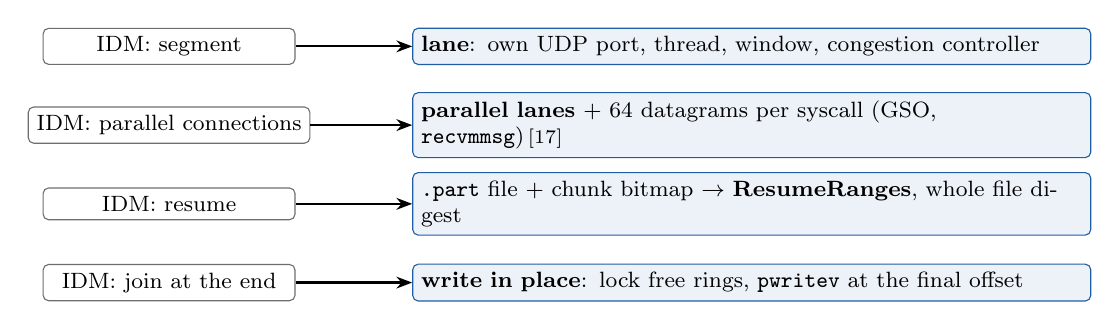
\begin{tikzpicture}[row sep=2mm]
    \foreach \y/\l/\r in {
      1.5/segment/{\textbf{lane}: own UDP port, thread, window, congestion controller},
      0.5/parallel connections/{\textbf{parallel lanes} + 64 datagrams per syscall (GSO, \texttt{recvmmsg})\rf{17}},
      -0.5/resume/{\texttt{.part} file + chunk bitmap $\rightarrow$ \textbf{ResumeRanges}, whole file digest},
      -1.5/join at the end/{\textbf{write in place}: lock free rings, \texttt{pwritev} at the final offset}} {
      \node[box, minimum width=3.2cm] (l) at (0,\y) {IDM: \l};
      \node[bbox, minimum width=8.6cm, text width=8.4cm, align=left] (r) at (7.4,\y) {\r};
      \draw[arr] (l) -- (r);
    }
  \end{tikzpicture}
  \vspace{4mm}

  \small Unlike IDM over TCP, every lane is a \textbf{reliable stream built on UDP blocks}: our own sequence
  numbers, selective ACKs, NACKs and timers, so there is no head of line blocking between lanes.
\end{frame}

% 7 ------------------------------------------------------------------------------------------------
\begin{frame}{Connection flow: handshake, setup, data transfer}
  \begin{columns}[T]
    \column{0.55\textwidth}
    \centering
    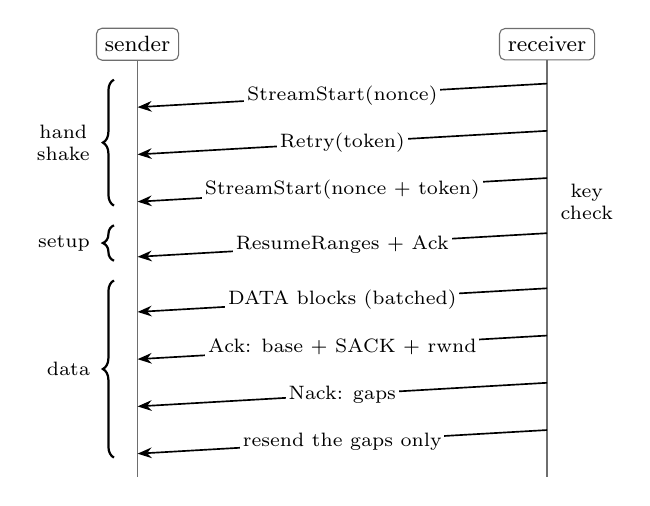
\begin{tikzpicture}[yscale=0.5, every node/.style={font=\scriptsize}]
      \node[box] at (0.9,0.7) {sender}; \node[box] at (6.1,0.7) {receiver};
      \draw[fgray] (0.9,0.3) -- (0.9,-10.3); \draw[fgray] (6.1,0.3) -- (6.1,-10.3);
      \foreach \y/\d/\t in {-0.3/r/StreamStart(nonce), -1.5/l/Retry(token), -2.7/r/StreamStart(nonce + token),
                            -4.1/l/ResumeRanges + Ack, -5.5/r/DATA blocks (batched), -6.7/l/Ack: base + SACK + rwnd,
                            -7.9/l/Nack: gaps, -9.1/r/resend the gaps only} {
        \ifx r\d \draw[msg] (0.9,\y) -- (6.1,\y-0.6); \else \draw[msg] (6.1,\y) -- (0.9,\y-0.6); \fi
        \node[fill=white, inner sep=1pt] at (3.5,\y-0.3) {\t};
      }
      \node[right, lab] at (6.15,-3.3) {key\\check};
      \draw[decorate, decoration={brace, amplitude=4pt, mirror}, thick] (0.6,-0.2) -- node[left=5pt, lab]{hand\\shake} (0.6,-3.4);
      \draw[decorate, decoration={brace, amplitude=4pt, mirror}, thick] (0.6,-3.9) -- node[left=5pt, lab]{setup} (0.6,-4.8);
      \draw[decorate, decoration={brace, amplitude=4pt, mirror}, thick] (0.6,-5.3) -- node[left=5pt, lab]{data} (0.6,-9.8);
    \end{tikzpicture}
    \column{0.43\textwidth}
    \happening{The sender proves it owns its address (echoes the \textbf{Retry} token) and that it holds the key
      (signed StreamStart). The receiver replies with the byte ranges it still needs; data then flows,
      acknowledged cumulatively and selectively.}
    \better{Each lane has its own window. Nothing is allocated before the peer is proven, so no amplification. A
      wrong key fails at the handshake. Resume is part of setup, not an extra.}
  \end{columns}
\end{frame}

% 8 ------------------------------------------------------------------------------------------------
\begin{frame}{Edge cases while data flows: sender side and receiver side}
  \begin{columns}[T]
    \column{0.49\textwidth}
    \centering\textbf{\small Sender side: an ACK is lost}\\[1mm]
    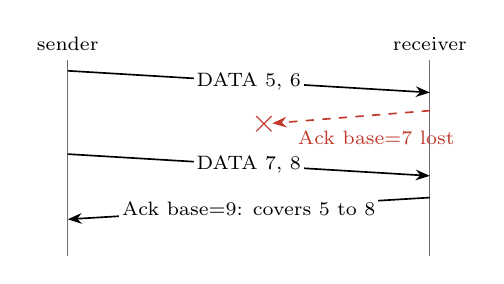
\begin{tikzpicture}[yscale=0.46, every node/.style={font=\scriptsize}]
      \draw[fgray] (0,0) -- (0,-5.4); \draw[fgray] (4.6,0) -- (4.6,-5.4);
      \node at (0,0.45) {sender}; \node at (4.6,0.45) {receiver};
      \draw[msg] (0,-0.3) -- (4.6,-0.9); \node[fill=white, inner sep=1pt] at (2.3,-0.6) {DATA 5, 6};
      \draw[lost] (4.6,-1.4) -- (2.6,-1.75); \node[fred] at (2.5,-1.77) {\large$\times$};
      \node[fred, right] at (2.8,-2.15) {Ack base=7 lost};
      \draw[msg] (0,-2.6) -- (4.6,-3.2); \node[fill=white, inner sep=1pt] at (2.3,-2.9) {DATA 7, 8};
      \draw[msg] (4.6,-3.8) -- (0,-4.4); \node[fill=white, inner sep=1pt] at (2.3,-4.1) {Ack base=9: covers 5 to 8};
    \end{tikzpicture}\\[-1mm]
    \scriptsize All ACKs lost? The RTO, $\max(\mathrm{SRTT}{+}4\,\mathrm{RTTVAR},\,2\,\mathrm{SRTT})$\rf{7}, resends the base +
    known holes, then backs off.
    \column{0.49\textwidth}
    \centering\textbf{\small Receiver side: a DATA block is lost}\\[1mm]
    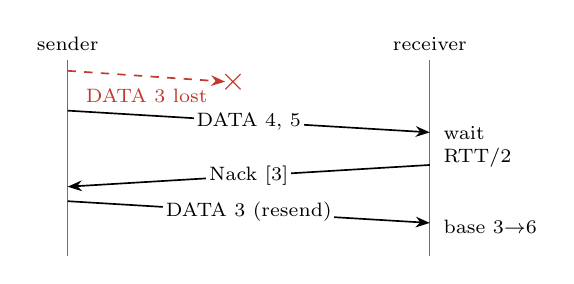
\begin{tikzpicture}[yscale=0.46, every node/.style={font=\scriptsize}]
      \draw[fgray] (0,0) -- (0,-5.4); \draw[fgray] (4.6,0) -- (4.6,-5.4);
      \node at (0,0.45) {sender}; \node at (4.6,0.45) {receiver};
      \draw[lost] (0,-0.3) -- (2.0,-0.6); \node[fred] at (2.1,-0.62) {\large$\times$};
      \node[fred, left] at (1.9,-1.0) {DATA 3 lost};
      \draw[msg] (0,-1.4) -- (4.6,-2.0); \node[fill=white, inner sep=1pt] at (2.3,-1.7) {DATA 4, 5};
      \node[right, align=left] at (4.65,-2.4) {wait\\RTT/2};
      \draw[msg] (4.6,-2.9) -- (0,-3.5); \node[fill=white, inner sep=1pt] at (2.3,-3.2) {Nack [3]};
      \draw[msg] (0,-3.9) -- (4.6,-4.5); \node[fill=white, inner sep=1pt] at (2.3,-4.2) {DATA 3 (resend)};
      \node[right] at (4.65,-4.6) {base 3$\to$6};
    \end{tikzpicture}\\[-1mm]
    \scriptsize Nack lost? Nack again after 1.5\,RTT. Duplicates and far ahead blocks are dropped.
  \end{columns}
  \vspace{1mm}
  \begin{columns}[T]
    \column{0.49\textwidth}\happening{ACKs are cumulative and carry a 1024 bit SACK map\rf{6}, so the next ACK repairs a lost one.}
    \column{0.49\textwidth}\better{A late block is not treated as lost: no spurious resends under reordering (QUIC: $\approx$1\,MB/s).}
  \end{columns}
\end{frame}

% 9 ------------------------------------------------------------------------------------------------
\begin{frame}{Edge cases in the handshake}
  \begin{columns}[T]
    \column{0.6\textwidth}
    \scriptsize
    \begin{tabular}{@{}p{0.34\linewidth}p{0.62\linewidth}@{}}
      \toprule
      \textbf{Case} & \textbf{What Fuse does} \\
      \midrule
      StreamStart / Retry lost & resend with backoff 1, 2, 4 \dots\ 200\,ms until the connect timeout \\
      Ack / ResumeRanges lost & the retried StreamStart (same nonce) makes the receiver resend them \\
      Stale Ack, old session & ignored: the nonce does not match \\
      Wrong or missing key & StreamStart fails authentication: \texttt{AuthFailed} at once \\
      Spoofed source address & gets only a 20 byte Retry; nothing is allocated \\
      Peer on another version & answered with a version reply (only a hint) \\
      \bottomrule
    \end{tabular}
    \column{0.38\textwidth}
    \centering
    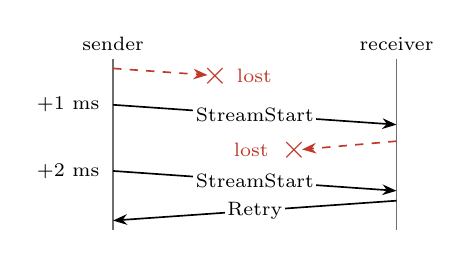
\begin{tikzpicture}[yscale=0.42, every node/.style={font=\scriptsize}]
      \draw[fgray] (0,0) -- (0,-5.2); \draw[fgray] (3.6,0) -- (3.6,-5.2);
      \node at (0,0.45) {sender}; \node at (3.6,0.45) {receiver};
      \draw[lost] (0,-0.3) -- (1.2,-0.5); \node[fred] at (1.3,-0.52) {\large$\times$}; \node[fred, right] at (1.45,-0.52) {lost};
      \node[left] at (-0.05,-1.4) {+1 ms};
      \draw[msg] (0,-1.4) -- (3.6,-2.0); \node[fill=white, inner sep=1pt] at (1.8,-1.7) {StreamStart};
      \draw[lost] (3.6,-2.5) -- (2.4,-2.75); \node[fred] at (2.3,-2.77) {\large$\times$}; \node[fred, left] at (2.1,-2.77) {lost};
      \node[left] at (-0.05,-3.4) {+2 ms};
      \draw[msg] (0,-3.4) -- (3.6,-4.0); \node[fill=white, inner sep=1pt] at (1.8,-3.7) {StreamStart};
      \draw[msg] (3.6,-4.3) -- (0,-4.9); \node[fill=white, inner sep=1pt] at (1.8,-4.6) {Retry};
    \end{tikzpicture}
  \end{columns}
  \vspace{2mm}
  \begin{columns}[T]
    \column{0.49\textwidth}\happening{Every handshake message is retried on silence, and every reply carries the sender's random nonce.}
    \column{0.49\textwidth}\better{Bounded by time, not a retry count, so it works at any RTT; a key or version problem is reported, not a timeout.}
  \end{columns}
\end{frame}

% 10 -----------------------------------------------------------------------------------------------
\begin{frame}{Inside the sender and the receiver}
  \begin{columns}[T]
    \column{0.44\textwidth}
    \centering\textbf{\small Sender: packet registry}\\[1mm]
    \fitwidth{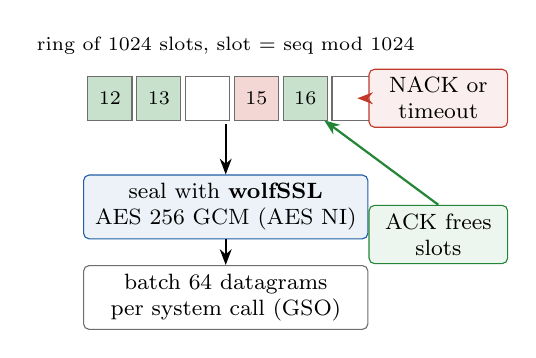
\begin{tikzpicture}[every node/.style={font=\scriptsize}]
      \foreach \i/\c in {0/fgreen!25,1/fgreen!25,2/white,3/fred!20,4/fgreen!25,5/white} {
        \draw[fill=\c, draw=fgray] (\i*0.62,0) rectangle ++(0.56,0.56);
      }
      \node at (0.28,0.28) {12}; \node at (0.9,0.28) {13}; \node at (2.14,0.28) {15}; \node at (2.76,0.28) {16};
      \node[align=center] at (1.75,0.95) {ring of 1024 slots, slot $=$ seq mod 1024};
      \node[bbox, text width=3.4cm] (seal) at (1.75,-1.1) {seal with \textbf{wolfSSL}\\AES 256 GCM (AES NI)};
      \node[box, text width=3.4cm] (gso) at (1.75,-2.25) {batch 64 datagrams\\per system call (GSO)};
      \draw[arr] (1.75,-0.05) -- (seal); \draw[arr] (seal) -- (gso);
      \node[rbox, text width=1.55cm] (nk) at (4.45,0.28) {NACK or\\timeout};
      \draw[arr, fred] (nk.west) -- (3.42,0.28);
      \node[gbox, text width=1.55cm] (ak) at (4.45,-1.45) {ACK frees\\slots};
      \draw[arr, fgreen] (ak.north) -- (3.0,0.0);
    \end{tikzpicture}}\\[1mm]
    \scriptsize every unacknowledged block is kept as an exact copy; a resend is byte identical
    \column{0.54\textwidth}
    \centering\textbf{\small Receiver: two separate paths}\\[1mm]
    \fitwidth{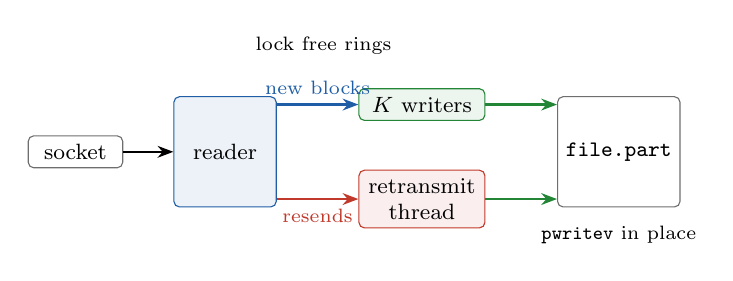
\begin{tikzpicture}[every node/.style={font=\scriptsize}]
      \node[box, minimum width=1.2cm] (s) at (0,0) {socket};
      \node[bbox, minimum width=1.3cm, minimum height=1.4cm] (r) at (1.9,0) {reader};
      \node[gbox, minimum width=1.6cm] (w) at (4.4,0.6) {$K$ writers};
      \node[rbox, minimum width=1.6cm] (rt) at (4.4,-0.6) {retransmit\\thread};
      \node[box, minimum width=1.5cm, minimum height=1.4cm] (f) at (6.9,0) {\texttt{file.part}};
      \draw[arr] (s) -- (r);
      \draw[arr, fblue] (r.east|-w) -- node[above]{new blocks} (w);
      \draw[arr, fred] (r.east|-rt) -- node[below]{resends} (rt);
      \draw[arr, fgreen] (w) -- (f.west|-w); \draw[arr, fgreen] (rt) -- (f.west|-rt);
      \node at (3.15,1.35) {lock free rings};
      \node at (6.9,-1.05) {\texttt{pwritev} in place};
    \end{tikzpicture}}\\[1mm]
    \scriptsize resends travel their own ring and thread, so recovery never waits behind new data;
    a full ring drops the block (NACK brings it back) instead of blocking the socket reader
  \end{columns}
  \vspace{3mm}
  \begin{columns}[T]
    \column{0.32\textwidth}\textbf{\small Lightweight crypto}\\\scriptsize wolfSSL (wolfCrypt): small C library, AES NI accelerated; no TLS stack on the data path
    \column{0.32\textwidth}\textbf{\small Big files}\\\scriptsize never held in memory; each block goes straight to its final offset
    \column{0.32\textwidth}\textbf{\small Resume}\\\scriptsize a chunk bitmap is saved every second; a rerun asks only for the missing ranges
  \end{columns}
\end{frame}

% 11 -----------------------------------------------------------------------------------------------
\begin{frame}{Connection close}
  \centering
  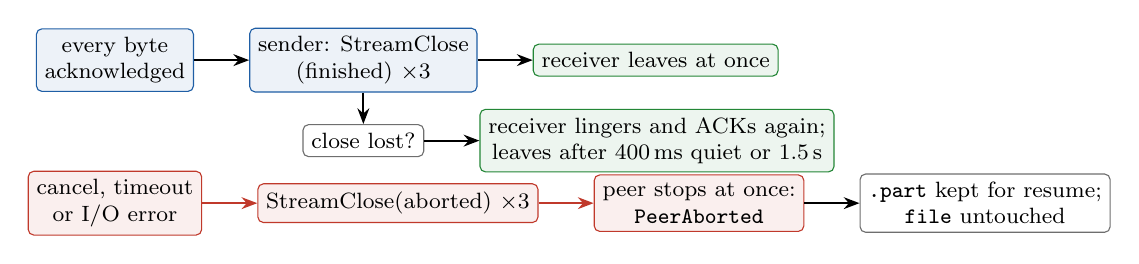
\begin{tikzpicture}[node distance=4mm and 7mm, every node/.style={font=\scriptsize}]
    \node[bbox] (a) {every byte\\acknowledged};
    \node[bbox, right=of a] (b) {sender: StreamClose\\(finished) $\times$3};
    \node[gbox, right=of b] (c) {receiver leaves at once};
    \node[box, below=of b] (d) {close lost?};
    \node[gbox, right=of d] (e) {receiver lingers and ACKs again;\\leaves after 400\,ms quiet or 1.5\,s};
    \draw[arr] (a) -- (b); \draw[arr] (b) -- (c); \draw[arr] (b) -- (d); \draw[arr] (d) -- (e);
    \node[rbox, below=10mm of a] (x) {cancel, timeout\\or I/O error};
    \node[rbox, right=of x] (y) {StreamClose(aborted) $\times$3};
    \node[rbox, right=of y] (z) {peer stops at once:\\\texttt{PeerAborted}};
    \node[box, right=of z] (p) {\texttt{.part} kept for resume;\\\texttt{file} untouched};
    \draw[arr, fred] (x) -- (y); \draw[arr, fred] (y) -- (z); \draw[arr] (z) -- (p);
  \end{tikzpicture}
  \vspace{4mm}
  \begin{columns}[T]
    \column{0.49\textwidth}\happening{A finished sender tells the receiver it may leave; an aborting side tells its peer. Both are sent three times and signed under a key.}
    \column{0.49\textwidth}\better{Neither side waits out a timeout, and the output file is either complete or untouched.}
  \end{columns}
\end{frame}

% 12 -----------------------------------------------------------------------------------------------
\begin{frame}{Results: throughput}
  \begin{columns}[T]
    \column{0.5\textwidth}
    \centering\small\textbf{Fuse vs QUIC} (quinn\rf{20}), 1 GiB file\\[-1mm]
    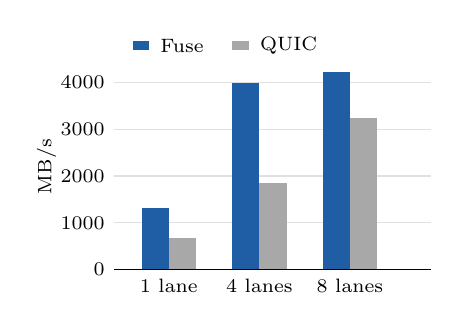
\begin{tikzpicture}[x=1.15cm, y=0.0006cm]
      \foreach \v in {0,1000,2000,3000,4000} {\draw[black!12] (0.4,\v) -- (3.9,\v); \node[lab, left] at (0.4,\v) {\v};}
      \foreach \i/\l/\f/\q in {1/1 lane/1327.7/678.6, 2/4 lanes/3980.8/1847.4, 3/8 lanes/4225.6/3238.4} {
        \fill[fblue] (\i-0.3,0) rectangle (\i,\f); \fill[fgray!60] (\i,0) rectangle (\i+0.3,\q);
        \node[lab, below] at (\i,0) {\l};
      }
      \draw (0.4,0) -- (3.9,0);
      \fill[fblue] (0.6,4700) rectangle ++(0.18,180); \node[lab, right] at (0.8,4790) {Fuse};
      \fill[fgray!60] (1.7,4700) rectangle ++(0.18,180); \node[lab, right] at (1.9,4790) {QUIC};
      \node[lab, rotate=90] at (-0.35,2200) {MB/s};
    \end{tikzpicture}\\
    \scriptsize 1.3 to 2.2$\times$ QUIC; 1.3 to 1.8$\times$ with encryption on both\\
    \scriptsize (repo benchmark, 16 core host, v5 to v7)
    \column{0.5\textwidth}
    \centering\small\textbf{Fuse vs TCP as the network gets worse}\\[-1mm]
    \fitwidth{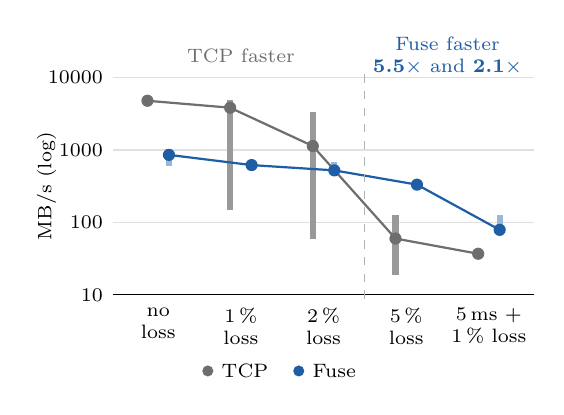
\begin{tikzpicture}[x=1.05cm, y=0.92cm]
      % log scale: y = log10(MB/s) - 1; medians from results.tex, bars span the 3 runs
      \foreach \v/\l in {0/10,1/100,2/1000,3/10000} {\draw[black!12] (0.45,\v) -- (5.55,\v); \node[lab, left] at (0.45,\v) {\l};}
      \node[lab, rotate=90] at (-0.35,1.5) {MB/s (log)};
      \draw[fgray!70, line width=2.2pt] (0.87,2.646) -- (0.87,2.703);
      \draw[fblue!45, line width=2.2pt] (1.13,1.786) -- (1.13,2.009);
      \node[lab, below, align=center] at (1,-0.05) {no\\loss};
      \draw[fgray!70, line width=2.2pt] (1.87,1.173) -- (1.87,2.697);
      \draw[fblue!45, line width=2.2pt] (2.13,1.737) -- (2.13,1.812);
      \node[lab, below, align=center] at (2,-0.05) {1\,\%\\loss};
      \draw[fgray!70, line width=2.2pt] (2.87,0.778) -- (2.87,2.530);
      \draw[fblue!45, line width=2.2pt] (3.13,1.681) -- (3.13,1.834);
      \node[lab, below, align=center] at (3,-0.05) {2\,\%\\loss};
      \draw[fgray!70, line width=2.2pt] (3.87,0.279) -- (3.87,1.107);
      \draw[fblue!45, line width=2.2pt] (4.13,1.500) -- (4.13,1.537);
      \node[lab, below, align=center] at (4,-0.05) {5\,\%\\loss};
      \draw[fgray!70, line width=2.2pt] (4.87,0.544) -- (4.87,0.602);
      \draw[fblue!45, line width=2.2pt] (5.13,0.833) -- (5.13,1.100);
      \node[lab, below, align=center] at (5,-0.05) {5\,ms +\\1\,\% loss};
      \draw[fgray, thick] (0.87,2.680) -- (1.87,2.584) -- (2.87,2.055) -- (3.87,0.778) -- (4.87,0.568);
      \draw[fblue, thick] (1.13,1.933) -- (2.13,1.792) -- (3.13,1.719) -- (4.13,1.522) -- (5.13,0.898);
      \fill[fgray] (0.87,2.680) circle (2.2pt);
      \fill[fgray] (1.87,2.584) circle (2.2pt);
      \fill[fgray] (2.87,2.055) circle (2.2pt);
      \fill[fgray] (3.87,0.778) circle (2.2pt);
      \fill[fgray] (4.87,0.568) circle (2.2pt);
      \fill[fblue] (1.13,1.933) circle (2.2pt);
      \fill[fblue] (2.13,1.792) circle (2.2pt);
      \fill[fblue] (3.13,1.719) circle (2.2pt);
      \fill[fblue] (4.13,1.522) circle (2.2pt);
      \fill[fblue] (5.13,0.898) circle (2.2pt);
      \draw (0.45,0) -- (5.55,0);
      \node[lab, text=fgray] at (2.0,3.3) {TCP faster};
      \node[lab, text=fblue, align=center] at (4.5,3.3) {Fuse faster\\\textbf{5.5$\times$} and \textbf{2.1$\times$}};
      \draw[black!30, dashed] (3.5,-0.05) -- (3.5,3.1);
      \fill[fgray] (1.6,-1.05) circle (2pt); \node[lab, right] at (1.65,-1.05) {TCP};
      \fill[fblue] (2.7,-1.05) circle (2pt); \node[lab, right] at (2.75,-1.05) {Fuse};
    \end{tikzpicture}}\\
    \scriptsize dot $=$ median, bar $=$ range of 3 runs; 4 vCPU VM, netem on loopback,\\
    \scriptsize 64\,MiB, 4 streams; every transfer intact.\\
    \scriptsize Fuse stays steady while TCP swings (2\,\% loss: \XTCPTWOLO\ to \XTCPTWOHI\,MB/s).
  \end{columns}
\end{frame}

% 13 -----------------------------------------------------------------------------------------------
\begin{frame}{Results: latency of small messages during a bulk transfer}
  \centering\footnotesize
  One way latency of 64 byte probes at 2000/s, idle and with 4 bulk streams running (\textmu s)\\[1mm]
  \begin{tabular}{@{}llrrl@{}}
    \toprule
    \textbf{Protocol} & \textbf{Configuration} & \textbf{p50} & \textbf{p99} & \\
    \midrule
    Fuse & idle & 14.1 & 39.6 & \multirow{5}{*}{\scriptsize repo, 16 core host} \\
    Fuse & under 6.3 GB/s bulk & \textbf{15.8} & \textbf{38.2} & \\
    QUIC & idle & 55.3 & 153.6 & \\
    QUIC & under bulk, same connection & 326.9 & \textcolor{fred}{\textbf{12584.8}} & $\times$82 \\
    QUIC & under bulk, separate connection & 42.5 & 82.4 & \\
    \midrule
    Fuse & idle & \FUSELATIDLEA & \FUSELATIDLEB & \multirow{5}{*}{\scriptsize this run, 12 core laptop} \\
    Fuse & under 5.5 GB/s bulk & \textbf{\FUSELATLOADA} & \textbf{\FUSELATLOADB} & \\
    TCP & idle & \TCPLATIDLEA & \TCPLATIDLEB & \\
    TCP & under bulk, same connection & \TCPLATSAMEA & \textcolor{fred}{\textbf{\TCPLATSAMEB}} & \\
    TCP & under bulk, separate connection & \TCPLATSEPA & \TCPLATSEPB & \\
    \bottomrule
  \end{tabular}
  \vspace{3mm}

  Fuse keeps telemetry latency \textbf{flat under load inside one session}; QUIC and TCP need a second
  connection (and handshake, and congestion controller) to get close.
\end{frame}

% 14 -----------------------------------------------------------------------------------------------
\begin{frame}{Results: reliability under a bad network}
  \begin{columns}[T]
    \column{0.55\textwidth}
    \scriptsize
    \begin{tabular}{@{}lrrc@{}}
      \toprule
      \textbf{Condition} (32 MiB) & \textbf{Fuse} & \textbf{QUIC} & \textbf{intact} \\
      \midrule
      clean relay & 2096 & 502 & both \\
      loss 2\,\% & 358 & 201 & both \\
      loss 5\,\% & 27 to 226 & 83 & both \\
      delay 25\,ms (50\,ms RTT) & 53 & 55 & both \\
      jitter 10\,$\pm$5\,ms & \textbf{50} & 0.6 & both \\
      reorder 10\,\% & \textbf{41} & 1.0 & both \\
      duplicate 3\,\% & 249 & 218 & both \\
      25\,ms RTT + 1\,\% loss & \textbf{52} & 2.8 & both \\
      \bottomrule
    \end{tabular}\\[1mm]
    MB/s through the \texttt{fuse\_netem} emulator\rf{18}; repo, 16 core host
    \column{0.42\textwidth}
    \centering\small\textbf{Bytes delivered intact}\\[1mm]
    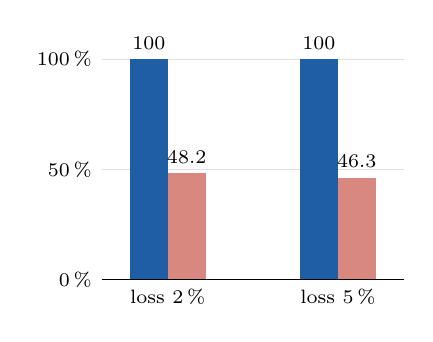
\begin{tikzpicture}[x=1.2cm, y=0.028cm]
      \foreach \v in {0,50,100} {\draw[black!12] (0.4,\v) -- (3.6,\v); \node[lab, left] at (0.4,\v) {\v\,\%};}
      \fill[fblue] (0.7,0) rectangle (1.1,100); \fill[fred!60] (1.1,0) rectangle (1.5,\UDPDELTWO);
      \fill[fblue] (2.5,0) rectangle (2.9,100); \fill[fred!60] (2.9,0) rectangle (3.3,\UDPDELFIVE);
      \node[lab, below] at (1.1,0) {loss 2\,\%}; \node[lab, below] at (2.9,0) {loss 5\,\%};
      \node[lab, above] at (1.3,\UDPDELTWO) {\UDPDELTWO}; \node[lab, above] at (3.1,\UDPDELFIVE) {\UDPDELFIVE};
      \node[lab, above] at (0.9,100) {100}; \node[lab, above] at (2.7,100) {100};
      \draw (0.4,0) -- (3.6,0);
    \end{tikzpicture}\\
    \scriptsize\textcolor{fblue}{$\blacksquare$} Fuse: 100\,\%, byte identical (this run)\\
    \textcolor{fred!60}{$\blacksquare$} raw UDP at full speed: emulated loss \emph{plus} overflow (no congestion control)\\
    TCP: reliable by design; not measured under loss in this run
  \end{columns}
\end{frame}

% 15 -----------------------------------------------------------------------------------------------
\begin{frame}{Bonus: SDKs and the browser}
  \centering
  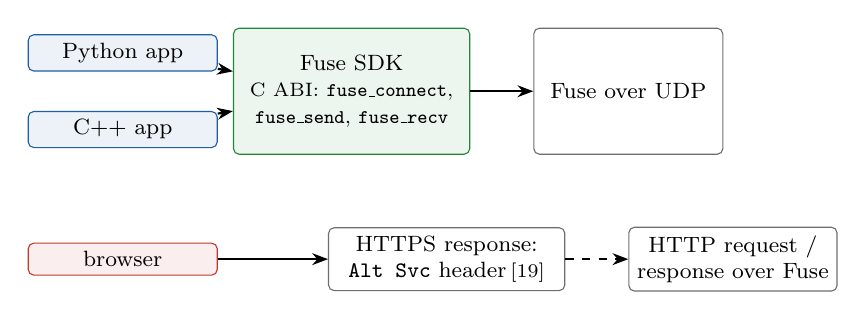
\begin{tikzpicture}[node distance=5mm and 8mm]
    \node[bbox, minimum width=2.4cm] (py) {Python app};
    \node[bbox, minimum width=2.4cm, below=of py] (cpp) {C++ app};
    \node[gbox, minimum width=3cm, minimum height=1.6cm, right=14mm of $(py)!0.5!(cpp)$] (sdk) {Fuse SDK\\\scriptsize C ABI: \texttt{fuse\_connect},\\\scriptsize \texttt{fuse\_send}, \texttt{fuse\_recv}};
    \node[box, minimum width=2.4cm, minimum height=1.6cm, right=of sdk] (net) {Fuse over UDP};
    \draw[arr] (py) -- (sdk); \draw[arr] (cpp) -- (sdk); \draw[arr] (sdk) -- (net);
    \node[rbox, minimum width=2.4cm, below=12mm of cpp] (br) {browser};
    \node[box, minimum width=3cm, right=14mm of br] (alt) {HTTPS response:\\\texttt{Alt Svc} header\rf{19}};
    \node[box, minimum width=2.4cm, right=of alt] (h) {HTTP request /\\response over Fuse};
    \draw[arr] (br) -- (alt); \draw[arr, dashed] (alt) -- (h);
  \end{tikzpicture}
  \vspace{3mm}
  \begin{columns}[T]
    \column{0.49\textwidth}\textbf{\small SDKs}\\\scriptsize Python and C++ bindings over the C API, \textbf{tested on macOS and Linux}; message oriented: what one \texttt{send} delivers, one \texttt{recv} returns
    \column{0.49\textwidth}\textbf{\small Browser (partial)}\\\scriptsize one HTTP/1.1 request and response per Fuse message, discovered through an \texttt{Alt Svc} header; validated headers, bounded server
  \end{columns}
\end{frame}

% 16 -----------------------------------------------------------------------------------------------
\begin{frame}{Demo}
  \centering
  \vspace{8mm}
  {\Huge Live demo}\\[6mm]
  {\large ncurses view of a Fuse transfer}\\[8mm]
  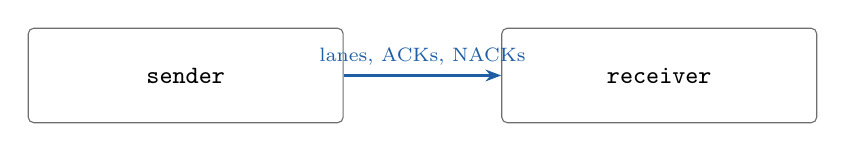
\begin{tikzpicture}
    \node[box, minimum width=4cm, minimum height=1.2cm, font=\ttfamily\small] (s) {sender};
    \node[box, minimum width=4cm, minimum height=1.2cm, font=\ttfamily\small, right=2cm of s] (r) {receiver};
    \draw[arr, fblue] (s) -- node[above, lab]{lanes, ACKs, NACKs} (r);
  \end{tikzpicture}
\end{frame}

% 17 -----------------------------------------------------------------------------------------------
\begin{frame}{Conclusion}
  \begin{itemize}
    \item \textbf{Problem:} a transport faster than QUIC with on par reliability, for telemetry \emph{and}
          large objects in one session
    \item \textbf{Idea:} IDM style parallel lanes, but every lane is its own reliable stream over UDP with its
          own congestion control
    \item \textbf{Protocol:} validated handshake, SACK + NACK recovery, write in place receiver with resume,
          clean close; hardened in two security reviews
    \item \textbf{Results:} 1.3 to 2.2$\times$ QUIC throughput; beats TCP under heavy loss and delay; flat small message latency under bulk load;
          byte identical delivery under loss, jitter and reordering
  \end{itemize}
  \vspace{6mm}
  \centering{\Large Thank you. Questions?}
\end{frame}

% 18-19 --------------------------------------------------------------------------------------------
\begin{frame}{References (1/2)}
  \scriptsize
  \begin{enumerate}[{[}1{]}]\setlength{\itemsep}{1pt}
    \item J.~Iyengar, M.~Thomson. \emph{QUIC: A UDP Based Multiplexed and Secure Transport}. RFC 9000, 2021.
    \item M.~Thomson, S.~Turner. \emph{Using TLS to Secure QUIC}. RFC 9001, 2021.
    \item J.~Iyengar, I.~Swett. \emph{QUIC Loss Detection and Congestion Control}. RFC 9002, 2021.
    \item W.~Eddy (Ed.). \emph{Transmission Control Protocol (TCP)}. RFC 9293, 2022.
    \item M.~Allman, V.~Paxson, E.~Blanton. \emph{TCP Congestion Control}. RFC 5681, 2009.
    \item M.~Mathis et al. \emph{TCP Selective Acknowledgment Options}. RFC 2018, 1996.
    \item V.~Paxson et al. \emph{Computing TCP's Retransmission Timer}. RFC 6298, 2011.
    \item G.~Fairhurst et al. \emph{Packetization Layer Path MTU Discovery for Datagram Transports}. RFC 8899, 2020.
    \item H.~Krawczyk, P.~Eronen. \emph{HMAC based Extract and Expand Key Derivation Function (HKDF)}. RFC 5869, 2010.
    \item E.~Rescorla. \emph{The Transport Layer Security (TLS) Protocol Version 1.3}. RFC 8446, 2018.
  \end{enumerate}
\end{frame}

\begin{frame}{References (2/2)}
  \scriptsize
  \begin{enumerate}[{[}1{]}]\setcounter{enumi}{10}\setlength{\itemsep}{1pt}
    \item M.~Dworkin. \emph{Recommendation for Block Cipher Modes of Operation: GCM and GMAC}. NIST SP 800 38D, 2007.
    \item A.~Joux. \emph{Authentication Failures in NIST version of GCM}. Comments to NIST, 2006.
    \item J.~P.~Aumasson, D.~J.~Bernstein. \emph{SipHash: a fast short input PRF}. INDOCRYPT 2012.
    \item V.~Jacobson. \emph{Congestion Avoidance and Control}. ACM SIGCOMM 1988.
    \item A.~Langley et al. \emph{The QUIC Transport Protocol: Design and Internet Scale Deployment}. ACM SIGCOMM 2017.
    \item IBM. \emph{Aspera FASP high speed transport} (product documentation).
    \item W.~de Bruijn, E.~Dumazet. \emph{Optimizing UDP for content delivery: GSO, pacing and zerocopy}. Linux Plumbers 2018; \texttt{recvmmsg(2)}.
    \item S.~Hemminger. \emph{Network Emulation with NetEm}. Linux Conf Australia, 2005.
    \item M.~Nottingham et al. \emph{HTTP Alternative Services}. RFC 7838, 2016; M.~Bishop. \emph{HTTP/3}. RFC 9114, 2022.
    \item Fuse project repository (GitHub, kamalkoushikd): \texttt{docs/PROTOCOL.md}, \texttt{bench/RESULTS.md}, project report; quinn QUIC implementation.
  \end{enumerate}
\end{frame}

% 20 -----------------------------------------------------------------------------------------------
\begin{frame}{Appendix: security hardening (protocol version 8)}
  \begin{columns}[T]
    \column{0.53\textwidth}
    \scriptsize
    \begin{tabular}{@{}p{0.33\linewidth}p{0.63\linewidth}@{}}
      \toprule
      \textbf{Problem (review)} & \textbf{Fix} \\
      \midrule
      AES GCM nonce reuse on resend\rf{11,12} & retransmit bit out of the AAD: a resend is identical \\
      Forged / replayed control & GMAC on every control message; replay window \\
      Spoofing, amplification & Retry token (SipHash\rf{13}); path validation \\
      Key overuse & lane keys rotate every $2^{22}$ blocks (HKDF\rf{9}) \\
      Unbounded size claims & \texttt{max\_receive\_bytes}; safe \texttt{.part} files \\
      Transport gaps & SACK, RFC 6298 RTO\rf{7}, slow start, pacing, flow control, MTU cap\rf{8} \\
      \bottomrule
    \end{tabular}
    \column{0.45\textwidth}
    \scriptsize
    \begin{tabular}{@{}lrl@{}}
      \toprule
      \textbf{Message} & \textbf{Bytes} & \textbf{Purpose} \\
      \midrule
      DATA & 31\,+\,n & block, offset, time \\
      ACK & 160 & base, SACK, rwnd \\
      NACK & 6\,+\,8n & missing blocks \\
      STREAM\_START & 80\,+\,e & size, salt, nonce \\
      RETRY & 20 & address token \\
      STREAM\_CLOSE & 13 & finished / aborted \\
      auth trailer & +24 & counter + GMAC \\
      \bottomrule
    \end{tabular}\\[2mm]
    220 tests pass (195 without crypto) in 4 build configurations.
  \end{columns}
  \vfill
  \centering\scriptsize
  \textbf{Full project report:}
  \href{https://github.com/kamalkoushikd/fuse-nw/blob/main/docs/report/report.pdf}{\texttt{github.com/kamalkoushikd/fuse-nw/blob/main/docs/report/report.pdf}}
\end{frame}

\end{document}
